\section{Virtualization}
Virtualization is a concept which is closely related to the one of Processes and multithreading, virtualization deals with extending or replacing an existing interface mimicing the behaviour of another system. \n
Virtualization is, nowadays, a standard; that is because it allows to handle hardware changes with ease because the hardware is virtualized and the interface does not change for the above system. With virtualization also come ease of portability and code migration and isolation of failing or attacked components. \n
There are different ways to do virtualization, a couple of interfaces to be virtualized are the following:
\begin{itemize}
    \item Instruction set architecture
    \item System calls
    \item Library calls
    \item Process virtualization in which we have a separate set of instructions, an interpreter/emulator, running atop an OS
    \item Native virtual machine monitor in which we have low level instructions along with barebones minimal operating system
    \item Hosted virtual machine monitor in which we have low level instructions but most of the work is delegated to a full fladged OS.
\end{itemize}
Now we will talk about virtualization and everything that revolves around it more in detail. \n
First virtualization is an activity aiming to create replacements for real resources, which have the same functionalities and external interfaces of their counterpart, but different attributes. \n
The concept of emulation and simulation are linked to virtualization, the three concepts mean different things. \n
\begin{itemize}
    \item Emulation: We execute a system like it is another system. We run os, API and functions on a machine which they have not been developed for.
    \item Simulation: An application allowing to execute old programs defined for different platforms on modern machines and it replicates the behaviour of a system. It's like a software emulation. \n
    Emulation is slower but precise while simulation is fast but less precise. We use simulation (or software emulation, to run old games on our smartphones).
    \item High level emulation is an intermediate between emulation and simulation, they recreate the functionalities of an emulated system using similar or equivalent functions in the emulating system.
    \item Virtualization: the technique for using resources and devices in a functional way without considering their physical layout. \n
    In the world of virtualization a Virtual Machine is a container with software based CPU, RAM and HDD and network connection. We have a certain level of transparency because an OS or an application do not distinguish between a virtual and a physical machine.
\end{itemize}
\begin{figure}
    \centering
    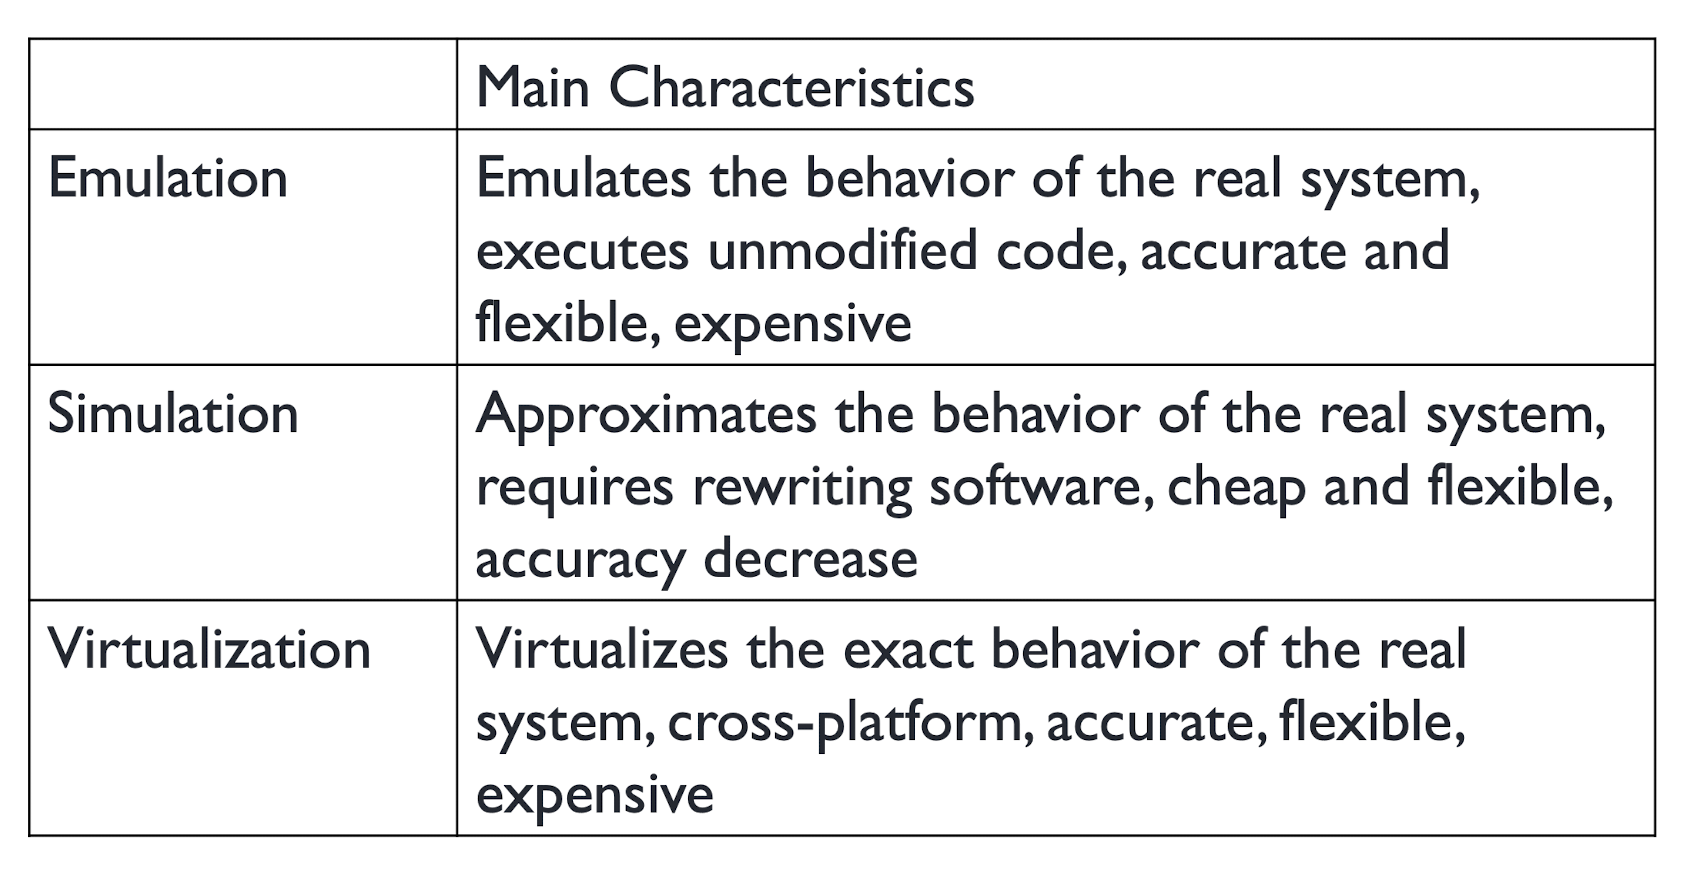
\includegraphics[scale=0.4]{./Images/summary_virtualization.png}
    \caption{Summary of the principal characteristics of virtualization techniques}
\end{figure}
Now we will focus on each one separately.
\subsection{Virtualization}
Virtualization is compatible with x86/64 machines, each has a full and dedicated environment and each machine is isolated from each other just like physical separation. \n
Virtualization was created to solve some issues:
\begin{itemize}
    \item Too many servers but small workloads
    \item Old hardware does not work
    \item Infrastructural requirements are always increasing (many independent servers)
    \item Small flexibility in shared environments
\end{itemize}
Virtualization allows to keep the costs low for resources while managing them efficiently and keeping the necessary computational power. We can, in fact, use a single hardware server as a multitude of virtual servers. \n
If a cloud solution has been deployed well we can use virtualization to increase resource usage and enable dynamic sharing of resource pools. We can even react to particular situations because virtualization allows us to have a single consolidated view of each resource of the network which can be easily accessed, moved and managed from wherever. \n
Other reasons that support the choice of going virtualized are the following:
\begin{itemize}
    \item Better performance
    \item transparency
    \item Heterogeneity
    \item portability
    \item Interoperability
    \item Green IT (with the same amount of hardware we satisfy more people)
\end{itemize}
Virtualization can be used in many different scenarios, it's heavily used in cloud-based applications because we can, for example, virtualize resources into pools and assign them to users based on the fee they pay and on their workload. \n
We can also use virtualization to deploy microservice-based applications by putting every microservice into its own virtualized container. \n
As a last example we can use virtualization to keep our systems secure, with a virtualized environment we can test code and / or applications to see that they work / do not contain viruses before downloading them on our own machine. \n
A couple of reasons against virtualization are the follwing:
\begin{itemize}
    \item Analysis and planning: building an application or a service that stands on top of a virtualized environment is easy enough, porting something to a virtualized environment a completely different workflow. A lot of planning and study has to go into the process, the staff needs to be trained and a lot of risk analysis has to be done.
    \item Adaptation and post adaptation: A lof of evaluation needs to go into studying the relaiability, the performance, the efficiency and the security of the virtualized environment that will be used.
    \item Maintenance: Maintenance must be kept in mind as well, mostly scalability and security.
\end{itemize}
\begin{figure}
    \centering
    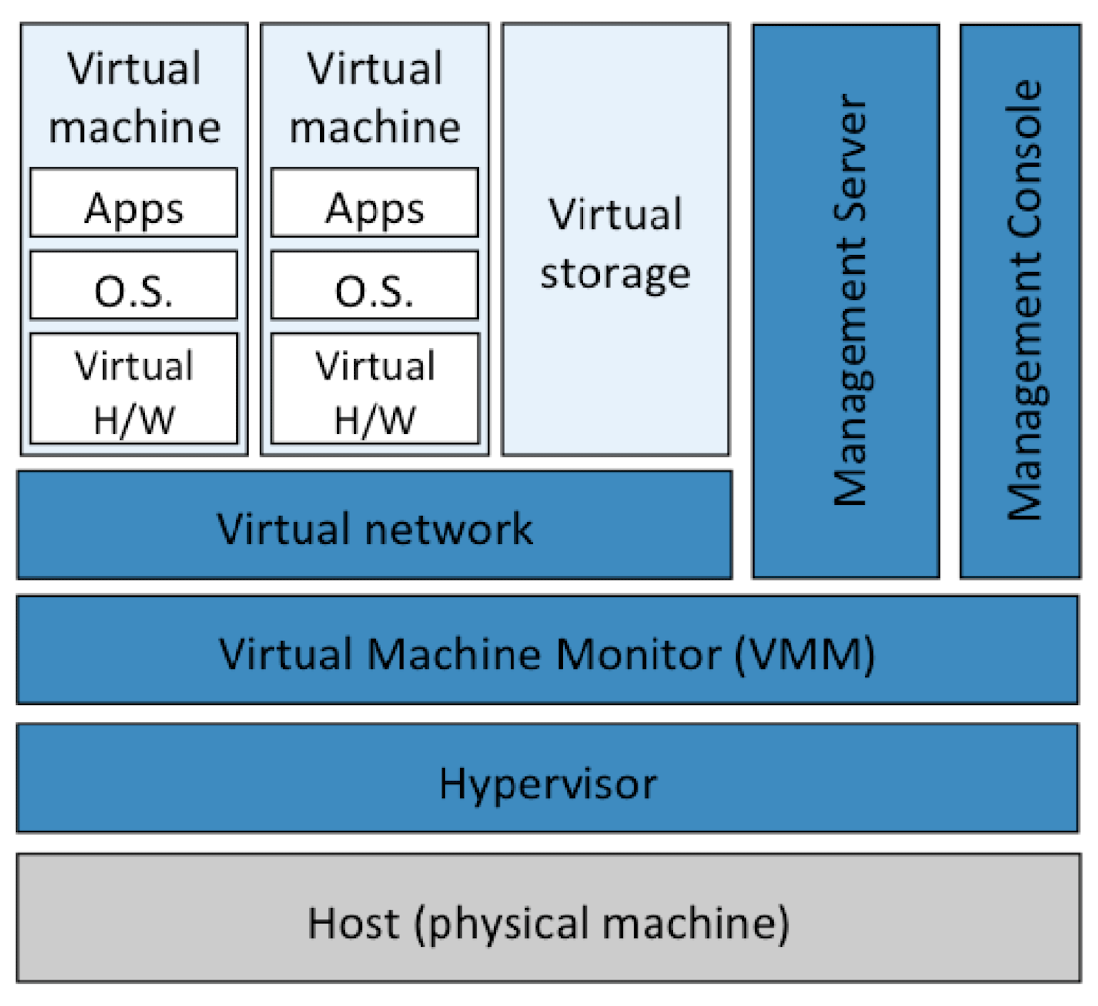
\includegraphics[scale=0.4]{./Images/virtualization_components.png}
    \caption{The structure of a virtualizer}
\end{figure}
Now we'll take a look at the structure of a virtualizer. \n
The components are the following: \n
\smallSpace
\textbf{Hypervisor} \n
The Hypervisor is a component that interacts with the virtual machine and with the host, it allows for multiple OSs running on the same computer. Beware! In the case of an operating system like windows it's important to keep in mind that turning on the Hypervisor and having a virtual machine manager like Virtual Box or VMware may cause instabilities. \n
\smallSpace
\textbf{Virtual machine monitor}\n
It's the application component realizing virtualization. \n
\smallSpace
\textbf{Guest OS} \n
\smallSpace
\textbf{Host OS} \n
\smallSpace
\textbf{management Server} \n
It's a virtualization platform.
\smallSpace
\textbf{Management Console} \n
Provides access to the virtualization management interface. \n
\subSpace
A cool factoid about virtualization is that there is a non-mandatory constraint that requires that a statistically relevant percentage of instructions inside a virtualized environment should be executed without virtualization. Abiding to this rule will guarantee better efficiency of the virtual machine. \n
Now we will consider a couple of different virtualization models. 
\begin{figure}
    \centering
    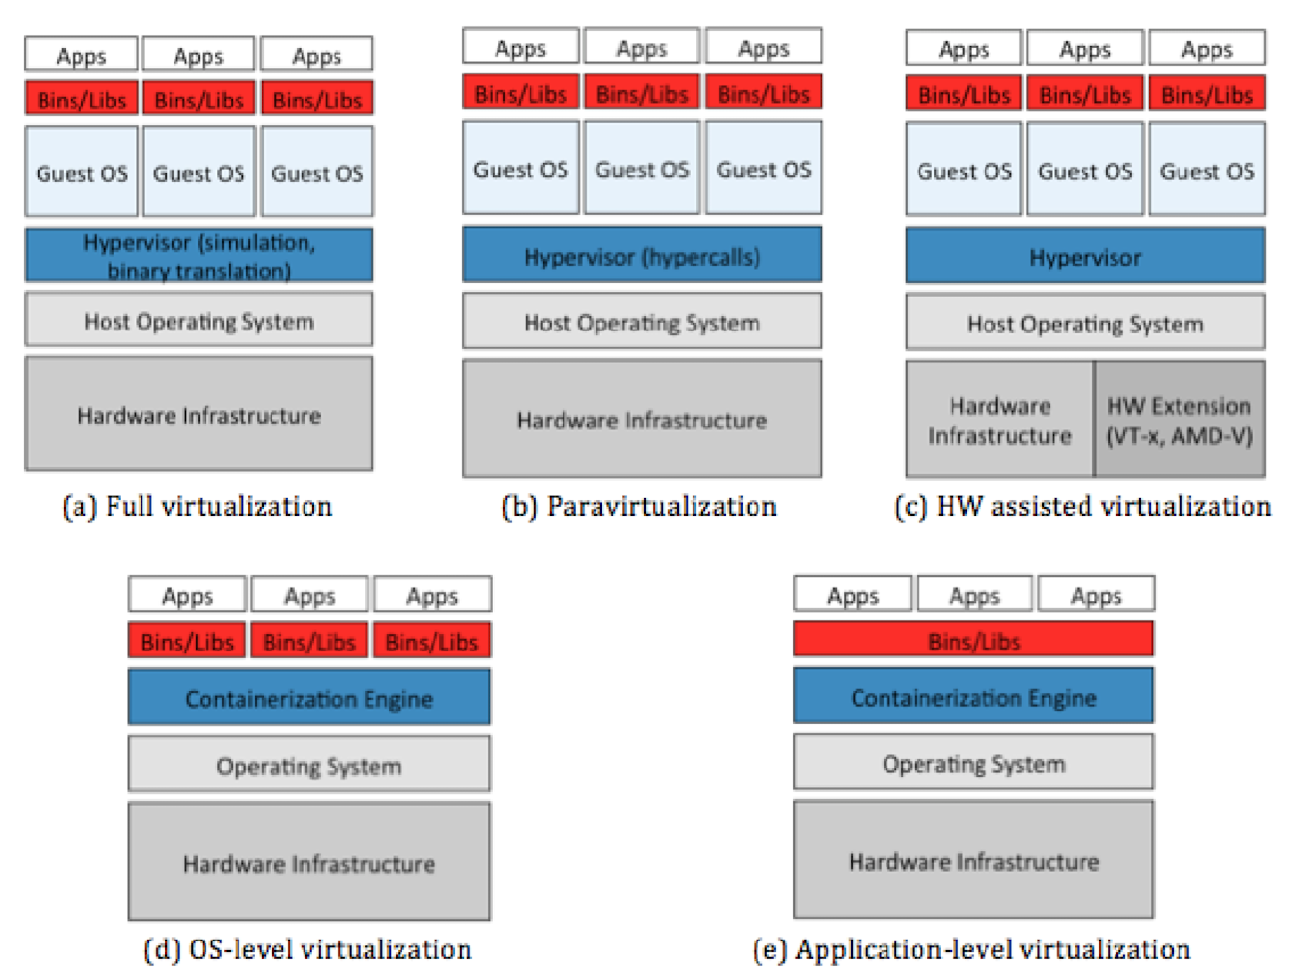
\includegraphics[scale=0.4]{./Images/virtualization_stacks.png}
    \caption{Various virtualization models}
\end{figure}
When doing \textbf{Full emulation}, we emulate every aspect of a computer and it allows to execute an unmodified guest OS on a completely different host architecture. \n
\miniSpace
\textbf{Full virtualization} [4a], instead, only emulates the necessary hardware, allowing the isolated execution of a guest OS, the only difference is that the guest OS must be designed for the same architecture. \n
\miniSpace
If we need to run software for MIPS-32 architecture we are going to need to emulate the whole machine because we cannot run a virtual machine made for something like that on x86. \n
\miniSpace
Nowadays processors come with instructions that allow to provide the virtual machine with some true hardware (\textbf{Hardware assisted virtualization} [4c]). That boosts machine performance with full virtualization. \n
\miniSpace
\textbf{Paravirtualization} [4b] is another form of virtualization where the virtual machine makes available an API to extend the guest OS (the guest OS has to be modified), the extension consists of hypercall implementation which is a virtualized version of a system call. Basically it's a way of opening a direct line of communication between the Guest OS and the Hypervisor below. \n
\miniSpace
In \textbf{OS-level virtualization} [4d] the virtual machine manager partitions hardware resources of host OS between the guests. The host OS guarantees the isolation of multiple user space instances. \n
\miniSpace
In \textbf{Application level virtualization} [4e] we have a virtualized application that runs in a safe and enclosed environment, this avoids risky memory overwrites that may break the operating system. This also allows for better portability of code. \n
\smallSpace
Virtualization can either be native or non-native, if it's native is fast because guest OS and host OS coincide and, probably, the Hypervisor is very low level and very efficient. In the other case we are working with a slower form of virtualization but it allows to have different operating systems. \n

\subsection{Virtualization Software}
Now we will se a couple of specific solutions for hardware virtualization.
\subsubsection{VMware ESXi}
The first virtualization platform that we'll check out is vSphere, which is an ecosystem including different virtualization solutions.
\begin{figure}
    \centering
    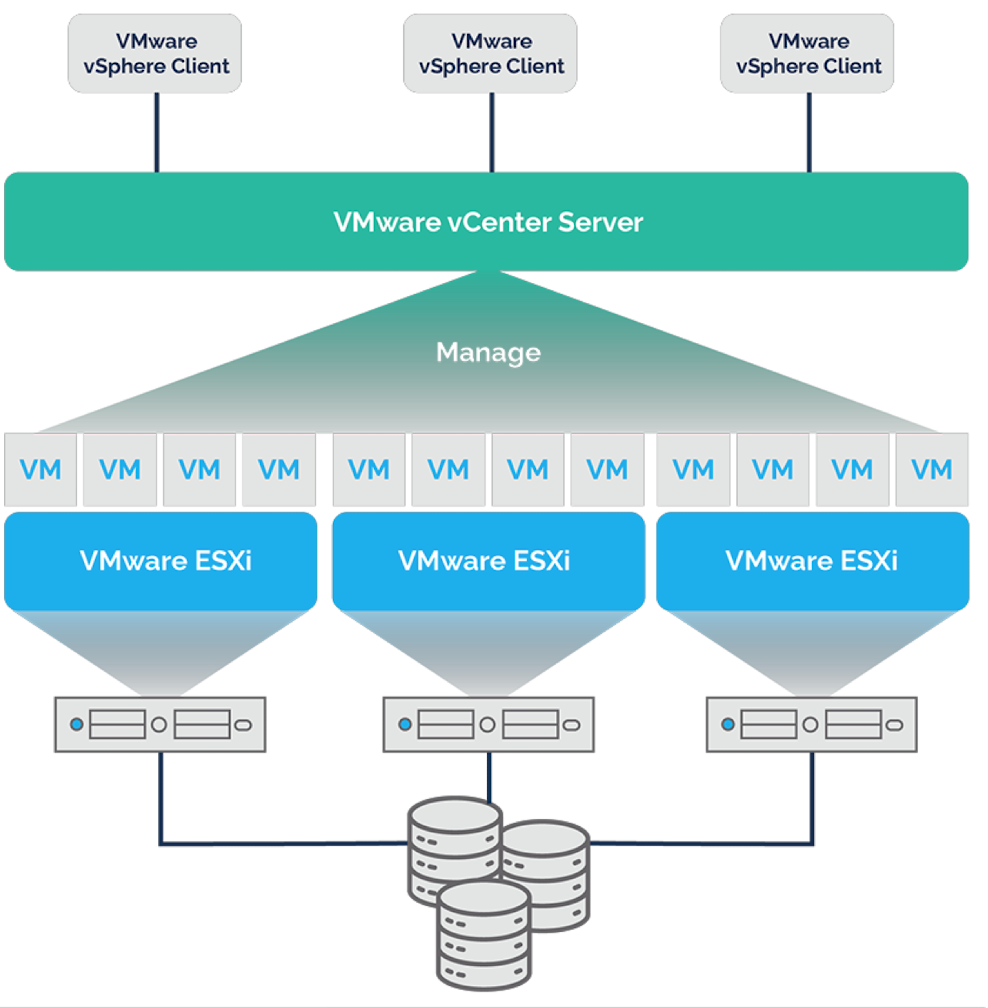
\includegraphics[scale=0.4]{Images/ESXi.png}
    \caption{VMware vSphere}
\end{figure}
vCenter is a management middleware layied on top of the virtualized environment and basically allows full control over the resources. This solution allows to control up to 2000 hosts and 35000 virtual machines. \n
ESXi is the vSphere's hypervisor and gives the fundamentals to build and manage a virtualized IT infrastructure. It's a bare-metal hypervisor, installed directly on server hardware and takes up only 150MB. It partitions the physical server into sveral virtual servers, each virtual machine is a complete system on its own. \n
Virtual machines can be kept safe via powerful encryption systems and role based access control.
\subsubsection{Xen}
Xen is a Paravirtualization hypervisor released under GPL2 license, with paravirtualization we can expect performance similar to a non-virtualized machine. It can scale up to monstrous numbers: 4095 host CPUs with 16TB of RAM; it's important to note that using paravirtualization the hypervisor supports a maximum of 512 VCPUs with 512GB of RAM per guest, while using Hardware Virtualization, it supports a maximum of 128 VCPUs and 1TB of RAM per guest. \n
Why should we use Xen?
\begin{itemize}
    \item It's reliable.
    \item It's flexible.
    \item It has a very good support for a wide range of operating systems and cloud platforms.
    \item It's secure because of the minimal attack surface.
    \item It's modular.
\end{itemize}
Xen is built on a very good and efficient hypervisor that allows strong isolation between components.
\subsubsection{KVM}
KVM is a full virtualization solution for Linux on x86 hardware, it's based on extensions supporting virtualization and can execute unmodified Linux or Windows images.
\subsection{Virtual Desktop}
Another very cool use of virtualization is virtual desktop, in this case we basically have remote resources and users can hop into a personal virtual machine just by using a thin client and their own credentials. If on one side we should have a completely seemless desktop experience that should present no differences from a user's prospective, on the other end the provider should be able to guarantee load balance, high availability, scalability and performance for all of its users. \n
The pros are the following:
\begin{itemize}
    \item Centralized management and security.
    \item Business continuity.
    \item Isolation and standard way of managing ProcessDecreases the need to buy new hardware.
    \item Decreases the time of adding a new image.
    \item Centralized adiminstration of all desktop, eventually located anywhere in the world.
\end{itemize}
Virtual desktop can be implemented in a varieties of ways dependeing on the type of solution / service desired. \n
\textbf{Single remote desktop} \n
In single remote desktop we basically remote into our own PC, it's widely used by IT management companies to handle problems on remote machines. \n
\miniSpace
\textbf{Shared Desktops} \n
Shared desktops are based upon a server hosting desktop users and applictaions, desktop sharing is widely used because all the computing power is located on a server and only the monitor, keyboard and mouse are connected to the network. \n
This system allows a centralized management of desktops and their applications, simplifying licensing and making easier to solve problems, because user applications are located on the server and not on several machines. \n
\miniSpace
\textbf{Blade physical desktops}
Users have their own PC, but the physical hardware is a blade PC located in a datacenter. The main pros and cons of this approach are the following:
\begin{itemize}
    \item Each user has his own PC, instead of sharing resources with other users.
    \item Terminal servers hosting shared desktops can be influenced by server faults/problems.
    \item Blades require more maintenance.
\end{itemize}
\textbf{Virtual Desktop} \n
A virtual desktop is the opposite of a shared desktop, a single client -PC or notebook- hosts multiple desktops, each one with its own operating system.
\subsection{Server Virtualization}
Server virtualization decreases the total cost of ownership because it allows to serve more clients with the same amount of computational power. It also allows to increase server usage and simplifies management via:
\begin{itemize}
    \item Dynamic provisioning
    \item Workload managment and isolation
    \item Virtual machine migration
    \item Reconfiguration
\end{itemize}